\section{Modularity and extensibility}

\begin{figure}[ht]
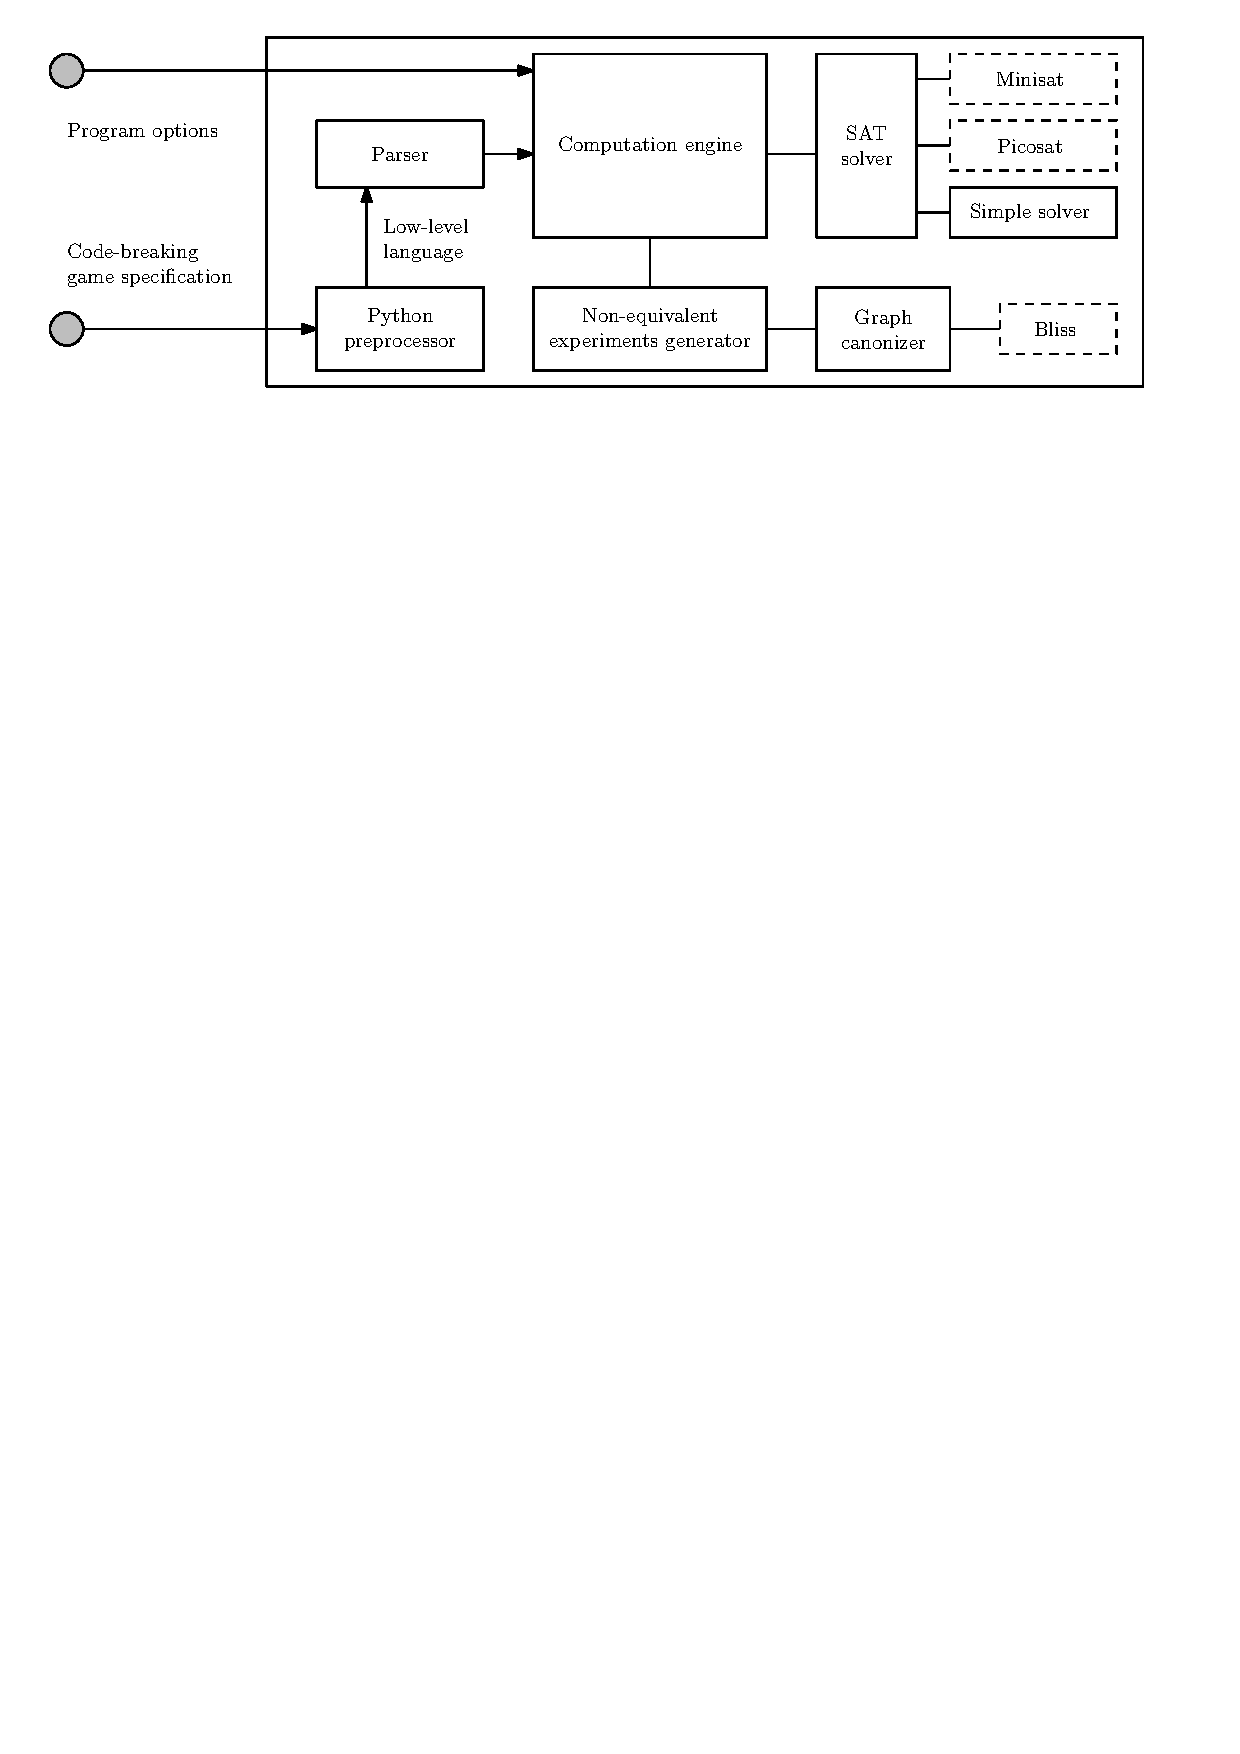
\includegraphics[width=\textwidth]{pictures/modularity.pdf}
\caption{Component diagram of Cobra.}
\label{fig:components}
\end{figure}


Cobra uses several external tools for SAT solving and graph canonization.
Nowadays, many high-performance SAT solvers are available
  and multiple tools for graph canonization exist.
Cobra was developed so that other external tools with the same functionality
  can be easily integrated.
\autoref{fig:components} shows a component diagram of
  the modular design of Cobra.

To integrate another SAT solver,
  create a new solver class that inherits from
  the abstract class \texttt{Solver} and
  implement all the necessary methods.
Details can be found in the \texttt{solver.h} file in the source codes
  and the required methods
  are described in the next section.

Cobra can also be easily extended with a new strategy for experiment selection.
The implementations of the supported strategies can be found in
  the \texttt{strategy.h} and \texttt{strategy.cpp} files.
To add a new strategy, create a corresponding function in this file
  and add an entry about the strategy
  to the \texttt{breaker\_strategies} table in \texttt{strategy.h}.
The strategy function should take a list of experiments
  as its only argument
  and return the index of the selected experiment in the list.

If the strategy is one-step look-ahead,
  you can use a provided template with a corresponding lambda function.
We demonstrate this possibility with a code snippet of
  the implementation of the ``exp-models'' strategy below.
For exact details, see the documentation in the source codes.

\begin{lstlisting}[language=C++]
uint breaker::exp_num(vec<Experiment>& list) {
  return minimize([](Experiment& e){
    uint sumsq = 0;
    for (uint i = 0; i < e.numOfOutcomes(); i++) {
      auto models = e.NumOfModelsOfOutcome(i);
      sumsq += models * models;
    }
    return static_cast<dobule>(sumsq) / e.TotalNumOfModels();
  }, list);
}
\end{lstlisting}

\section{SAT solving} \label{s:cobra-sat}

Cobra uses a SAT solver for the following tasks.
\begin{itemize}
\item Compute the total number of possible codes.
\item Verify that an experiment is well-formed (see \autoref{s:cobra-modes}).
\item Identify satisfiable outcomes of an experiment and disregard the others.
\item Decide whether the game is finished -- whether the accumulated
  knowledge as a formula has only one model.
\item Evaluate the strategies -- count models, fixed variables, etc.
\end{itemize}

Most of these tasks require an \emph{incremental SAT solver}, by which we mean a
  SAT solver that supports incremental adding and removing constraints.
Without this feature, we would have to call the solver from a clean state
  many times on the whole formula, which would ruin the computation time.

The solver must implement the following methods.
\begin{itemize}
\item \textsc{AddConstraint}(formula). Adds a constraint.
\item \textsc{Satisfiable()} $->$ Bool. Decides whether the current constraints are satisfiable.
\item \textsc{GetAssignment()} $->$ Assignment.
  After a successful \textsc{Satisfiable} call, this function retrieves
  the satisfying assignment from the solver.
\item \textsc{OpenContext(), CloseContext()}.
  \textsc{OpenContext} adds a context to a stack.
  Every call to \textsc{AddConstraint} adds the constraint to the context on the top of the stack.
  \textsc{CloseContext} removes all constraints in the current context and removes it
  from the stack. It must be possible to nest contexts arbitrarily.
  %The two methods are sometimes called just \textsc{Push} and \textsc{Pop}.
\item \textsc{HasOnlyOneModel()} $->$ Bool. Decides whether the current constraints have only one model.
  This can be done by asking whether the formula is satisfiable and if it is,
  retrieving the satisfying assignment, adding
  a constraint that rejects this assignment, and asking for satisfiability again.
  The pseudocode of this method is shown in \autoref{alg:onlyonemodel}.
  % Adding the new clause should be done in a new context in order not to pollute
  % the solver state.

\item \textsc{CountModels()} $->$ Int.
SAT solvers do not typically include support for model counting, the problem
  commonly referred to as \#SAT.
One solution is to use
  a special tool designed for this purpose,
  such as SharpSAT\footnote{\url{https://sites.google.com/site/marcthurley/sharpsat}}\cite{sharpsat}.
However, we have not found a model counting tool that supports incremental SAT solving.

% Second option is to use a SAT solver, repeatedly ask for satisfiability and
%   add clauses that forbids the current assignment until we get
%   an unsatisfiable formula. The pseudocode is shown in \autoref{alg:modelcounting2}.

Another option is to use an incremental SAT solver and a simple backtracking approach,
  progressively assuming a variable to be true or false and cutting the non-perspective
  (unsatisfiable) branches.
The pseudocode in the form of a recursive in shown \autoref{alg:modelcounting3},
  where the initial value of $X$ in the set of propositional variables.
\end{itemize}

\begin{algorithm}[ht]
\caption{Decision whether a formula has exactly one model}
\label{alg:onlyonemodel}
\DontPrintSemicolon
\lIf{not \textsc{Satisfiable()}}{\Return{false}}
$v <- $ \textsc{GetAssignment()}\;
\textsc{OpenContext()}\;
\textsc{AddConstraint($\overline{x_1}\| ... \|\overline{x_n}$)},
  where $\overline{x_i}$ is $\neg\:x_i$ if $v(x_i) = 1$ and $x_i$ otherwise\;
$sat <- $\textsc{Satisfiable()}\;
\textsc{CloseContext()}\;
\Return{$\neg sat$}
\end{algorithm}
% \begin{algorithm}[ht]
% \caption{Model counting, second option.}
% \label{alg:modelcounting2}
% \DontPrintSemicolon
% $models <- 0$\;
% \textsc{OpenContext()}\;
% \While{\textsc{Satisfiable()}} {
%   $v <- $ \textsc{GetAssignment()}\;
%   \textsc{AddConstraint($\overline{x_1}\| ... \|\overline{x_n}$)},
%     where $\overline{x_i}$ is $\neg\:x_i$ if $v(x_i) = 1$ and $x_i$ otherwise\;
%   $models <- models + 1$\;
% }
% \textsc{CloseContext()}\;
% \Return{$models$}
% \end{algorithm}
\begin{algorithm}[h!]
\caption{Model counting}
\label{alg:modelcounting3}
\DontPrintSemicolon
\SetKwProg{fun}{Function}{}{}
\fun{\textsc{Count}\textnormal{($X$)}}{
$models <- 0$\;
\lIf{$X = \emptyset$}{\Return{1}}
$x <- $ any variable from $X$\;
\textsc{OpenContext()}\;
\textsc{AddConstraint}($x$)\;
\lIf{\textsc{Satisfiable()}}{$models <- models \:+ $ \textsc{Count}($X\setminus \{x\}$)}
\textsc{CloseContext()}\;
\textsc{OpenContext()}\;
\textsc{AddConstraint}($\neg x$)\;
\lIf{\textsc{Satisfiable()}}{$models <- models \:+ $ \textsc{Count}($X\setminus \{x\}$)}
\textsc{CloseContext()}\;
\Return{$models$}
}{}
\end{algorithm}

Cobra includes three SAT solver implementations that are described next.

\subsection{PicoSat}
Picosat\footnote{\url{http://fmv.jku.at/picosat/}} \cite{picosat} is a simple,
  extensible SAT solver, which supports incremental SAT solving exactly in the way
  we need.
Picosat is available under the \emph{MIT License}.

Bindings to Picosat are implemented in the \texttt{PicoSolver} class.
This class also implements the model counting algorithm \ref{alg:modelcounting3}
 as Picosat does not support model counting itself.

\subsection{MiniSat}

Minisat\footnote{\url{http://minisat.se/}} \cite{minisat} is a minimalistic,
  extensible SAT solver, which won several SAT competitions in the past.
Minisat is also available under the \emph{MIT License}.

Minisat does not support incremental SAT solving in the manner we described
  but it supports ``assumptions''.
You can assume arbitrary number of unit clauses
  (i.e. that a variable is true of false) and ask for satisfiability under
  these assumptions.

The behaviour we need can be simulated by the assumptions in the following way.
For each context, we create a new variable, say $a$.
Then, instead of adding clauses $C_1, C_2, ..., C_n$ to the context,
  we add clauses $\{\neg a, C_1\}$, $\{\neg a, C_2\}$, ... $\{\neg a, C_n\}$ and ask
  for satisfiability under the assumption $a$ (in general,
  under the assumption that all variables corresponding
  to the open contexts are true).
Afterwards, when a context is closed, we add a unit clause $\{\neg a\}$,
  which effectively removes all the clauses in the context.
% The only minor issue with this approach is that the variable $a$ is wasted,
%   the solver will remember it somewhere and may consume more memory.

Bindings to Minisat are implemented in the \texttt{MiniSolver} class.
This class implements the context opening and closing in the way described above
  and the model counting algorithm \ref{alg:modelcounting3}.

\subsection{Simple solver}

We include a special SAT solver, called \texttt{SimpleSolver} to
  compare the proper SAT solvers with a simple approach based on model enumeration.
Simple solver uses another SAT solver (Minisat) to generate all
  models of the first constraint, which is carried out in the same way
  as model counting described above.

Satisfiability questions with additional constraint are
  resolved by going though all possible codes (assignments) and
  checking that the constraints are satisfied.
Model counting and the other functions are implemented similarly.

Note that Simple solver is optimized for context opening and closing.
It remembers which models become unsatisfied in which contexts and
  adds them back to the list of possibilities when the context is closed.

\subsection{Transformation to CNF}

The input formula for a SAT solver must be typically specified
  in the conjunctive normal form (CNF).
Since we do not have such requirement for formulas in our input format,
  and since we allow non-standard numerical operators,
  we need to transform a formula to CNF first.

The standard transformation works as follows.
First, we express the formula in a form
  that uses only negations, conjunctions and disjunctions.
Then, we transform the formula to \emph{negation normal form} using De Morgan's laws
  and, finally, we use distributivity of conjunction and disjunction to
  move all conjunctions to the top level.
This procedure may lead to exponential explosion of the formula, so
another solution, called \emph{Tseitin transformation}, is commonly used
  for transformation of a formula to CNF\cite{tseitin}.

Imagine the input formula as a circuit with gates corresponding to the logical operators.
Input vectors correspond to variable assignments and the circuit output
  is true if and only if the input assignment satisfies the formula.
For each gate, a new variable representing its output is created.
The resulting formula is a conjunction of subformulas that enforce
  the proper operation of the gates.

For example, consider an AND gate, inputs of which corresponds to variables
  $x$, $y$ and output corresponds to a variable $w$.
We need to ensure that $w$ is true if and only if both $x$ and $y$ are true,
  which is done by adding a subformula $w <-> (x \wedge y)$, which can be
  expressed in CNF as
\[
(\neg x \vee \neg y \vee w) \wedge
(x \vee \neg w) \wedge
(y \vee \neg w).
\]

Other gate types are handled similarly and this is done for all gates in the circuit.
Finally, the variable
  corresponding to the result of the top level operator is added
  to the resulting formula as a unit clause.

It remains to explain how we handle the numerical operators
  $\atleast$, $\atmost$ and $\exactly$.
We show the transformation of $\exactlyk{k}(f_1, ..., f_n)$,
  the other operators are transformed analogically.
For simplicity,
  assume $f_i$ are variables; if not, we take the variable corresponding the
  the subformulas.

For each $l\in\{0,1,...,k\}$ and $m\in\{1,...,n\}$, $l <= m$, we create
  a new variable $z_{l,\:m}$ which will be true if and only if
  the formula $\exactlyk{l}(f_1, ..., f_m)$ is satisfied.
To enforce this assignment, we add subformulas
  \[ z_{l,\:m} <-> (f_m \wedge z_{l-1,\:m-1}) \vee (\neg f_m \wedge z_{l,\:m-1}) \]
  for each $l > 1$, $m > 1$ (in CNF).
Special cases $l = m$ and $l = 0$ are equivalent to
  a conjunction and to a conjunction of the negated variables, respectively,
  and are transformed accordingly.

The size of the resulting subformula is linear in $n\cdot k$.
Although this is not polynomial in the size of the input
  (supposing $k$ is encoded in binary form)
  it is much better than a naive solution
  that expresses the formula as a conjunction of
  the $n\choose k$ possibilities,
  which would be double exponential.

\section{Graph isomorphism}

To implement the suggested method for detection of equivalent experiments,
  we need a method to decide whether two given graphs are isomorphic.
This problem is famous for not being proven either P-complete or
  NP-complete, so no polynomial algorithm for the problem is known.
However, software tools are available for graph canonization,
  which are quite efficient for sparse graphs and can be used to
  decide graph isomorphism by comparison of the canonical forms of the graphs.

Nauty\footnote{\url{http://pallini.di.uniroma1.it}}\cite{nauty} and
  Bliss\footnote{\url{http://www.tcs.hut.fi/software/bliss}}\cite{bliss}
  are the most well-known tools for this purpose.
These programs are primarily designed to compute automorphism groups of graphs
  but they can produce a canonical labelling of the graph as well.
For various reasons including simple integration, we decided to use Bliss,
  which is available under the \emph{GNU GPL v3} license.

For comparison of Nauty and Bliss,
  there are several benchmarks on the Nauty's website and
  we recommend an overview of the algorithms used by these tools
   in \cite{nautyblissoverview}.


\section{Implementation details} \label{sec:impl}

\subsection{Programming language and style}

Since the problems we attempt to solve are computationally very demanding,
  we had to choose a high-performing programming language.
Since the external tools we use are written in C and C++,
  a natural choice of a language for our tool was C++.
Cobra is written in the latest standard of the language, C++11, which
  contains significant changes both in the language and in the standard libraries
  and, in our opinion, improves readability and programmer's efficiency
  compared to previous versions.

We wanted the style of our code to be consistent and to use
  the language in the best manner possible according to industrial practice.
From the wide range of style guides available online
  we chose \emph{Google C++ Style Guide}\cite{googlestyle} and made
  the code compliant with all its rules except for a few exception.
The only significant violation are lambda functions, which are forbidden
  due to various reasons
  but we think that they are more beneficial than harmful in this project.

\subsection{Requirements}

The usage of a modern programming language requires
  a modern compiler that supports all the C++11 features we use.
We have successfully tested compilation with
 \texttt{gcc} version $4.8.2$ and
 \texttt{clang} version $3.2$.
For the Python preprocessing, the Python interpreter version $2.6$ or higher is required.

The tool is platform independent.
We have been able to successfully compile and test the functionality of the tool
  on Linux (Ubuntu 14.04) and Mac OS X (10.9).

\subsection{Testing}
Correctness is automatically a top priority for a tool of this kind so
  we implemented two automatic testing methods to
  capture potential programmer's error as soon as possible.

Unit testing has became a popular part of software development process
  in the last decades and is very effective for testing the functionality
  of particular modules and functions.
From the large amount of unit test frameworks available for C++,
  we have chosen \emph{Google Test}\footnote{\url{https://code.google.com/p/googletest/}},
  because of its simplicity, minimal amount of work needed to add new tests
  and very good assertion support.
The unit tests are automatically compiled and executed if you run \texttt{make utest}
  in the tool directory.

Functional tests provide a great method to test end-to-end functionality
  of the software.
These tests execute the program on sample inputs and compare the output
  with their expectations.
We have implemented several functional tests for the most common
  operations.
They can be run by \texttt{make ftest} in the tool directory.
